% По умолчанию используется шрифт 14 размера. Если нужен 12-й шрифт, уберите опцию [14pt]
\documentclass[14pt
  , russian
  %, xcolor={svgnames}
  ]{matmex-diploma-custom}
\usepackage[table]{xcolor}
\usepackage{graphicx}
\usepackage{tabularx}
\newcolumntype{Y}{>{\centering\arraybackslash}X}
\usepackage{amsmath}
\usepackage{amsthm}
\usepackage{amsfonts}
\usepackage{amssymb}
\usepackage{mathtools}
\usepackage{thmtools}
\usepackage{thm-restate}
\usepackage{tikz}
\usepackage{wrapfig}
% \usepackage[kpsewhich,newfloat]{minted}
% \usemintedstyle{vs}
\usepackage[inline]{enumitem}
\usepackage{subcaption}
\usepackage{caption}
\usepackage[nocompress]{cite}
\usepackage{makecell}
% \setitemize{noitemsep,topsep=0pt,parsep=0pt,partopsep=0pt}
% \setenumerate{noitemsep,topsep=0pt,parsep=0pt,partopsep=0pt}


\graphicspath{ {resources/} }

% 
% % \documentclass 
% %   [ a4paper        % (Predefined, but who knows...)
% %   , draft,         % Show bad things.
% %   , 12pt           % Font size.
% %   , pagesize,      % Writes the paper size at special areas in DVI or
% %                    % PDF file. Recommended for use.
% %   , parskip=half   % Paragraphs: noindent + gap.
% %   , numbers=enddot % Pointed numbers.
% %   , BCOR=5mm       % Binding size correction.
% %   , submission
% %   , copyright
% %   , creativecommons 
% %   ]{eptcs}
% % \providecommand{\event}{ML 2018}  % Name of the event you are submitting to
% % \usepackage{breakurl}             % Not needed if you use pdflatex only.
% 
% \usepackage{underscore}           % Only needed if you use pdflatex.
% 
% \usepackage{booktabs}
% \usepackage{amssymb}
% \usepackage{amsmath}
% \usepackage{mathrsfs}
% \usepackage{mathtools}
% \usepackage{multirow}
% \usepackage{indentfirst}
% \usepackage{verbatim}
% \usepackage{amsmath, amssymb}
% \usepackage{graphicx}
% \usepackage{xcolor}
% \usepackage{url}
% \usepackage{stmaryrd}
% \usepackage{xspace}
% \usepackage{comment}
% \usepackage{wrapfig}
% \usepackage[caption=false]{subfig}
% \usepackage{placeins}
% \usepackage{tabularx}
% \usepackage{ragged2e}
% \usepackage{soul}
\usepackage{csquotes}
% \usepackage{inconsolata}
% 
% \usepackage{polyglossia}   % Babel replacement for XeTeX
%   \setdefaultlanguage[spelling=modern]{russian}
%   \setotherlanguage{english}
% \usepackage{fontspec}    % Provides an automatic and unified interface 
%                          % for loading fonts.
% \usepackage{xunicode}    % Generate Unicode chars from accented glyphs.
% \usepackage{xltxtra}     % "Extras" for LaTeX users of XeTeX.
% \usepackage{xecyr}       % Help with Russian.
% 
% %% Fonts
% \defaultfontfeatures{Mapping=tex-text}
% \setmainfont{CMU Serif}
% \setsansfont{CMU Sans Serif}
% \setmonofont{CMU Typewriter Text}

\usepackage[final]{listings}

\lstdefinelanguage{ocaml}{
keywords={@type, function, fun, let, in, match, with, when, class, type,
nonrec, object, method, of, rec, repeat, until, while, not, do, done, as, val, inherit, and,
new, module, sig, deriving, datatype, struct, if, then, else, open, private, virtual, include, success, failure,
lazy, assert, true, false, end},
sensitive=true,
commentstyle=\small\itshape\ttfamily,
keywordstyle=\ttfamily\bfseries, %\underbar,
identifierstyle=\ttfamily,
basewidth={0.5em,0.5em},
columns=fixed,
fontadjust=true,
literate={->}{{$\to$}}3 {===}{{$\equiv$}}1 {=/=}{{$\not\equiv$}}1 {|>}{{$\triangleright$}}3 {\\/}{{$\vee$}}2 {/\\}{{$\wedge$}}2 {>=}{{$\ge$}}1 {<=}{{$\le$}} 1,
morecomment=[s]{(*}{*)}
}

\lstset{
mathescape=true,
%basicstyle=\small,
identifierstyle=\ttfamily,
keywordstyle=\bfseries,
commentstyle=\scriptsize\rmfamily,
basewidth={0.5em,0.5em},
fontadjust=true,
language=ocaml
}
 
\newcommand{\cd}[1]{\texttt{#1}}
\newcommand{\inbr}[1]{\left<#1\right>}


\newcolumntype{L}[1]{>{\raggedright\let\newline\\\arraybackslash\hspace{0pt}}m{#1}}
\newcolumntype{C}[1]{>{\centering\let\newline\\\arraybackslash\hspace{0pt}}m{#1}}
\newcolumntype{R}[1]{>{\raggedleft\let\newline\\\arraybackslash\hspace{0pt}}m{#1}}



\usepackage{soul}
\usepackage[normalem]{ulem}
%\sout{Hello World}

% перевод заголовков в листингах
\renewcommand\lstlistingname{Листинг}
\renewcommand\lstlistlistingname{Листинги}

\usepackage{afterpage}
\usepackage{pdflscape}
% TODO: Понять, почему я выделил то, что тут в отдельный файл
\usepackage{listings}
\usepackage{tikz}
\usetikzlibrary{decorations.pathreplacing,calc,shapes,positioning,tikzmark}

\newcounter{tmkcount}

\tikzset{
  use tikzmark/.style={
    remember picture,
    overlay,
    execute at end picture={
      \stepcounter{tmkcount}
    },
  },
  tikzmark suffix={-\thetmkcount}
}

\usepackage{ amssymb }
\usepackage[utf8]{inputenc}
\usepackage{babel}
\usepackage{amsthm}
\usepackage{algorithm}
\usepackage{multicol, multirow}

\usepackage{amsmath}
\usepackage{fancyvrb}
\usepackage{tikz}
\usepackage{pgfplots}
\usepackage{fontawesome}

\usetikzlibrary{automata, positioning, shapes,arrows}

\usepackage[caption=false]{subfig}
\usepackage{minted}
\usepackage{sidecap} 
\usepackage{fancyvrb}
\usepackage{wrapfig}
\usepackage{graphicx}
\usepackage{float}
\usepackage{color, colortbl}

\usepackage[noend]{algpseudocode}

\usepackage{hyperref}

\renewcommand{\labelitemii}{$ $}

\definecolor{green}{RGB}{34, 189, 65}

\theoremstyle{definition}
\newtheorem{definition}{Определение}[section]

\begin{document}
%% Если что-то забыли, при компиляции будут ошибки Undefined control sequence \my@title@<что забыли>@ru
%% Если англоязычная титульная страница не нужна, то ее можно просто удалить.
\filltitle{ru}{
    %% Актуально только для курсовых/практик. ВКР защищаются не на кафедре а в ГЭК по направлению, 
    %%   и к моменту защиты вы будете уже не в группе.
    chair              = {Кафедра системного программирования},
    group              = {19Б.10-мм},
    %
    %% Макрос filltitle ненавидит пустые строки, поэтому обязателен хотя бы символ комментария на строке
    %% Актуально всем.
    title              = {Разработка алгоритма для задачи достижимости с регулярными ограничениями},
    % 
    %% Здесь указывается тип работы. Возможные значения:
    %%   coursework - отчёт по курсовой работе;
    %%   practice - отчёт по учебной практике;
    %%   prediploma - отчёт по преддипломной практике;
    %%   master - ВКР магистра;
    %%   bachelor - ВКР бакалавра.
    type               = {practice},
    %
    %% Здесь указывается вид работы. От вида работы зависят критерии оценивания.
    %%   solution - <<Решение>>. Обучающемуся поручили найти способ решения проблемы в области разработки программного обеспечения или теоретической информатики с учётом набора ограничений.
    %%   experiment - <<Эксперимент>>. Обучающемуся поручили изучить возможности, достоинства и недостатки новой технологии, платформы, языка и т. д. на примере какой-то задачи.
    %%   production - <<Производственное задание>>. Автору поручили реализовать потенциально полезное программное обеспечение.
    %%   comparison - <<Сравнение>>. Обучающемуся поручили сравнить несколько существующих продуктов и/или подходов.
    %%   theoretical - <<Теоретическое исследование>>. Автору поручили доказать какое-то утверждение, исследовать свойства алгоритма и т.п., при этом не требуя написания кода.
    kind               = {solution},
    %
    author             = {Порсев Денис Витальевич},
    % 
    %% Актуально только для ВКР. Указывается код и название направления подготовки. Типичные примеры:
    %%   02.03.03 <<Математическое обеспечение и администрирование информационных систем>>
    %%   02.04.03 <<Математическое обеспечение и администрирование информационных систем>>
    %%   09.03.04 <<Программная инженерия>>
    %%   09.04.04 <<Программная инженерия>>
    %% Те, что с 03 в середине --- бакалавриат, с 04 --- магистратура.
    specialty          = {02.03.03 <<Математическое обеспечение и администрирование информационных систем>>},
    % 
    %% Актуально только для ВКР. Указывается шифр и название образовательной программы. Типичные примеры:
    %%   СВ.5006.2017 <<Математическое обеспечение и администрирование информационных систем>>
    %%   СВ.5162.2020 <<Технологии программирования>>
    %%   СВ.5080.2017 <<Программная инженерия>>
    %%   ВМ.5665.2019 <<Математическое обеспечение и администрирование информационных систем>>
    %%   ВМ.5666.2019 <<Программная инженерия>>
    %% Шифр и название программы можно посмотреть в учебном плане, по которому вы учитесь. 
    %% СВ.* --- бакалавриат, ВМ.* --- магистратура. В конце --- год поступления (не обязательно ваш, если вы были в академе/вылетали).
    programme          = {СВ.5006.2017 <<Математическое обеспечение и администрирование информационных систем>>},
    % 
    %% Актуально только для ВКР, только для матобеса и только 2017-2018 годов поступления. Указывается профиль подготовки, на котором вы учитесь.
    %% Названия профилей можно найти в учебном плане в списке дисциплин по выбору. На каком именно вы, вам должны были сказать после второго курса (можно уточнить в студотделе).
    %% Вот возможные вариканты:
    %%   Математические основы информатики
    %%   Информационные системы и базы данных
    %%   Параллельное программирование
    %%   Системное программирование
    %%   Технология программирования
    %%   Администрирование информационных систем
    %%   Реинжиниринг программного обеспечения
    % profile            = {Системное программирование},
    % 
    %% Актуально всем.
    %supervisorPosition = {проф. каф. СП, д.ф.-м.н., проф.}, % Терехов А.Н.
    supervisorPosition = {доцент кафедры информатики, к.ф.-м.н.,}, % Григорьев С.В.
    supervisor         = {Григорьев С.В.}
    % 

    % consultantPosition = {должность ООО <<Место работы>> степень},
    % consultant         = {К.К. Консультант}
}

\maketitle
\setcounter{tocdepth}{2}
\tableofcontents

% \begin{abstract}
%   В курсаче не нужен
% \end{abstract}

\section*{Введение}
\paragraph{}
Графы являются одной из основных структур в информатике, а алгоритмы над ними чрезвычайно важны в анализе компьютерных и социальных сетей, статическом анализе кода, биоинформатике~\cite{gb_math}. Графы, возникающие в данных областях, могут содержать миллионы узлов и ребер, поэтому распараллеливание алгоритмов для работы с ними оказывается необходимым условием достижения высокой производительности. Однако такое улучшение их эффективности происходит за счет более сложной модели программирования~\cite{blast}. Результатом этого становится, в том числе, несоответствие между языками высокого уровня, на которых пользователи и разработчики графовых алгоритмов предпочли бы программировать (например, Python), и языками программирования для параллельного оборудования~\cite{blast}. Таким образом, существующие решения либо просты в использовании (networkx\footnote{Репозиторий библиотеки networkx: \url{https://github.com/networkx/networkx}. Дата посещения: 13.12.2020}), либо высокопроизводительны (gunrock\footnote{Репозиторий библиотеки gunrock: \url{https://github.com/gunrock/gunrock} Дата посещения: 13.12.2020}). Проблемой является и то, что традиционные параллельные алгоритмы для анализа графов тяжело реализовывать и оптимизировать, а прирост производительности от роста числа параллельных процессов снижается~\cite{gb_math}. 

С появлением эффективных структур и алгоритмов для разреженных матриц становится возможным использование подхода к вычислению над графами, основанного на линейной алгебре. Матрица смежности может представлять широкий спектр графов, включая ориентированные, взвешенные, двудольные. Ключевым свойством такого подхода является способность оперировать богатым набором графов различных типов с помощью небольшого набора матричных операций над полукольцами. Например, транспонирование матрицы смежности изменяет направления ребер в ориентированном графе, а умножение матрицы на вектор, как показано на рисунке~\ref{fig:bfs_step}, является шагом в алгоритме поиска в ширину.

\begin{figure}[h!]
    \centering
    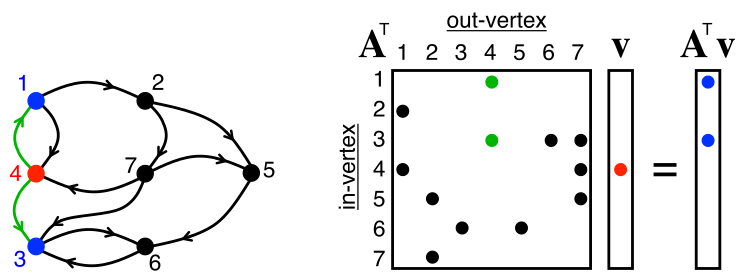
\includegraphics[width=0.9\linewidth]{pictures/MatrixBFS.png}
    \caption{Вычисление одного шага в алгоритме поиска в ширину\footnotemark}
    \label{fig:bfs_step}
\end{figure}

Спецификация GraphBLAS~\cite{gb_math} определяет базовые примитивы для построения графовых алгоритмов в терминах линейной алгебры. Разработчики считают, что эта область достаточно зрела, чтобы иметь потребность в стандартизации. Стандартизация позволяет сконцентрировать усилия исследователей на разработке инновационных алгоритмов для анализа и обработки графов, а не придумывать все новые, во многом пересекающиеся, низкоуровневые решения. Кроме того, благодаря такому подходу, по словам авторов\cite{sevengr}, возможно решение некоторых проблем, описанных ниже.
\begin{enumerate}
    \item \textbf{Переносимость.} Алгоритмы не требуют модификаций для достижения высокой производительности на конкретном устройстве.
    \item \textbf{Лаконичность.} Алгоритмы выражаются гораздо меньшим числом строчек кода.
    \item \textbf{Производительность.} Алгоритмы остаются высокопроизводительными.
    \item \textbf{Масштабируемость.} Алгоритмы эффективны как на небольших, так и на огромных данных.
\end{enumerate}

\footnotetext{GraphBLAS [Электронный ресурс] // Википедия. Свободная энциклопедия. – URL: \url{https://en.wikipedia.org/wiki/GraphBLAS} (дата обращения: 13.12.2020).}

GraphBLAS описывает небольшое множество математических операций, которые необходимы для реализации широкого спектра операций над графами. В стандарте описаны следующие объекты:
\begin{itemize}
    \item абстрактные структуры для хранения дынных (матрицы, векторы)
    \item алгебраические структуры (моноиды, полукольца, бинарные и унарные операторы)
    \item операции линейной алгебры над произвольными алгебраическими структурами (произведение матриц, поэлементное сложение и умножение, взятие подматрицы и т.д.)
    \item объекты управления (маски и дескрипторы)
\end{itemize}

На данный момент стандарт GraphBLAS уже имеет несколько полноценных реализаций\footnote{Форум, посвященный стандарту GraphBLAS: \url{https://graphblas.github.io/}. Дата посещения: 04.06.2021}, однако все они в основном ориентированы на исполнение на CPU. В то же время разработка инструмента с поддержкой исполнения на графических процессорах общего назначения является перспективным направлением исследований, так как их использование может существенно повысить производительность такого рода решений\cite{gbtl}\cite{blast}. На текущий момент нет стандартного подхода к реализации спецификации GraphBLAS на GPU --- разработчики сталкиваются не только с проблемами, связанными с реализацией обобщенных операций на графических процессорах с помощью стандартных инструментов языка C++, но и с переносимостью решений, основанных на программно-аппаратной платформе CUDA. Одним из возможных подходов к реализации GraphBLAS на GPU является использование языка высокого уровня, а также библиотек, динамически транслирующих конструкции и объекты данного языка в низкоуровневый код, способный исполнятся на графическом процессоре видеокарты. 


\section{Обзор}
\label{sec:relatedworks}
Рассмотрим алгоритмы, решающие задачу поиска путей с контекстно-свободными ограничениями с помощью операций линейной алгебры, в несколько этапов. Первым этапом приведем определения, встречающиеся в их описании. Вторым этапом рассмотрим алгоритм, основанный на произведении Кронекера, и алгоритм, основанный на матричном умножении, и сравним их, выделяя проблемы, которые лягут в основу работы. Последним этапом выберем инструмент для оценки производительности решений указанных проблем.
\subsection{Базовые определения}

Следующее определение формально описывает структуру представления грамматики для алгоритма, основанного на произведении Кронекера.
\theoremstyle{definition}
\begin{definition}
Рекурсивный автомат \cite{rec} над конечным алфавитом $\Sigma$ есть набор $(M,m,\{C_i\}_{i \in M})$, где 

\begin{itemize}
    \item $M$ конечное множество меток,
    \item $m \in M$ начальная метка,
    \item $ \{C_i\}_{i \in M} $ множество \textit{конечных автоматов},
          где $C_i=(\Sigma \cup M, Q_i,q_i^0,F_i,\delta_i)$:
    \begin{itemize}
        \item $\Sigma \cup M$ множество символов, $\Sigma \cap M = \emptyset$,
        \item $Q_i$ конечное множество состояний,
              где $Q_i \cap Q_j = \emptyset, \forall i \neq j$,
        \item $q_i^0$ начальное состояние $C_i$,
        \item $F_i$ множество финальных состояний $C_i$, где $F_i \subseteq Q_i$,
        \item $\delta_i$ функция переходов $C_i$,
              где $\delta_i: Q_i \times (\Sigma \cup M)
              \to Q_i$.
    \end{itemize}
\end{itemize}
\end{definition}

\begin{definition}
Пусть $\mathcal{G}$ = $( \Sigma, $N$, $P$, $S$ )$ --- контекстно-свободная грамматика, тогда $\mathcal{G}$ находится в \textbf{ослабленной нормальной форме Хомского} (ОНФХ), если содержит только правила вида:
\begin{itemize}
    \item $A \rightarrow BC$, где $A$, $B$, $C \in N$
    \item $A \rightarrow a$, где $A \in N$, $a \in \Sigma$
    \item $A \rightarrow \varepsilon$, где $A \in N$
\end{itemize}
\end{definition}

Определение ОНФХ отличается от нормальной формы Хомского наличием правил вида $A \rightarrow \varepsilon$, где А --- любой нетерминал, то есть А не обязательно является стартовым, а также допущением использовать стартовый нетерминал в правых частях правил при наличии правила вида $S \to \varepsilon$.

\begin{definition}
Пусть $G$ --- помеченный граф с n вершинами, $M$ --- матрица смежности $G$ и $L$ --- множество различных меток на дугах графа $G$, тогда матрицей смежности для $l \in L$ называется матрица $M^l$ размером $n \times n$, где 
\begin{equation*}
M^l[i, j] = \begin{cases} true \text{, между вершинами i и j существует дуга с меткой } $l$\\ false \text{, иначе} \end{cases}    
\end{equation*} 
\end{definition}

\subsection{Алгоритм, основанный на произведении Кронекера}

В статье~\cite{10.1007/978-3-030-54832-2_6} был представлен алгоритм, основанный на произведении Кронекера, для поиска путей между всеми парами вершин, именуемый алгоритмом построения индекса, то есть результатом работы является структура данных, указывающая между какими парами есть требуемый путь. Представленный алгоритм основан на матричных операциях и использует рекурсивный автомат.

Алгоритм (листинг 2) принимает граф $G$ и рекурсивный автомат $R$. Основная идея заключается в использовании произведения Кронекера, как инструмента для пересечения двух автоматов. В качестве второго автомата в алгоритме предлагается выбрать граф $G$. Такой выбор является корректным, так как каждую вершину можно считать состоянием, а дуги --- переходами.

На начальном этапе (строки 2-3) алгоритма берутся матрицы смежности для всех меток графа и автомата по определению 1.3. Стоит отметить, что определение 1.3 дано для графа, но аналогичное определение можно ввести и для рекурсивного автомата. Дополнительно (строки 4-5) для каждого нетерминала из $R$ создается пустая матрица смежности в наборе $M_2$, который соответствует графу $G$.

Первым шагом (строки 6-9) проверяется наличие состояний в автомате $R$, которые одновременно являются стартовыми и конечными, то есть проверяется наличие $\varepsilon$ правил для грамматики. При наличии таковых из каждой вершины в неё же есть искомый путь.

Основной цикл (строки 10-20) алгоритма выполняется до тех пор пока набор матриц смежности для графа меняется. Первым шагом цикла происходит вычисление произведения Кронекера (строка 11), тем самым создавая матрицу смежности нового автомата. Далее результат транзитивно замыкается для получения информации о достижимости состояний в полученном автомате. И последним шагом (строки 14-20) происходит обновление при помощи операций, представленных на листинге 1, матрицы графа, которая соответствует нетерминалу, конечное состояние автомата которого достижимо из начального состояния.

%Алгоритм (листинг 2) принимает граф G и рекурсивный автомат R. Операции выполняются с булевской декомпозицией матриц смежности входных данных. Такой вид представления требует соответствующее переопределение операций, то есть операцией умножения будет являться логическое И, а операцией сложения --- логическое ИЛИ. Алгоритм состоит из трёх последовательных операций: произведение Кронекера, транзитивное замыкание и обновление. Произведение Кронекера пересекает два автомата (R и G), его результат транзитивно замыкается и на шаге обновления добавляются дуги с метками в виде соответствующих нетерминалов. Шаги алгоритма повторяются пока граф изменяется. На каждой итерации находятся пути длиной (количество дуг) на один больше чем на предыдущей.

%Алгоритм построения индекса, основанный на тензорном произведении, был представлен в статье~\cite{10.1007/978-3-030-54832-2_6}, который в рамках работы для краткости будет называться просто алгоритмом, основанным на Кронекеровом произведении. Он основан на матричных операциях, что позволяет использовать при его реализации высокопроизводительные библиотеки линейной алгебры. А также данный алгоритм использует рекурсивный автомат для представления грамматки, что дает ему преимущество по сравенению с алгоритмом~\cite{alg_matrix}, основанным на матричном умножении, так как второй принимает на вход грамматику лишь в ОНФХ, что приводит к её разрастанию, и, как следствие, отрицательно сказывается на производительности. Однако в процессе работы алгоритма, основанного на Кронекеровом произведении, а именно в результате Кронекерова произведения, возникают матрицы больших размеров. Например, если указанным образом перемножить одну матрицу размером $m \times p$ и вторую матрицу $n \times q$, то в результате получается матрица $mn \times pq$, что может отрицательно сказаться на производительности.

%Рассмотрим алгоритм подробнее. Пусть (см. листинг 2) $M_{1}$ --- набор матриц смежности меток для рекурсивного автомата, а $M_{2}$ --- набор матриц смежности для $\mathcal{G}$. При таком подходе каждой метке соответствует булева матрица смежности, то есть для какой-то метки A $M_{1}[A][i,j] = true$ означает наличие ребра из i в j с меткой A. Такой вид представления требует соответствующее переопределение операций, то есть операцией умножения будет являться логическое И, а операцией сложения --- логическое ИЛИ. Перед началом основного цикла алгоритма происходит постановка дуг среди вершин, среди которых существует путь длины 0. На первом же шаге основного цикла вычисляется Кронекерово произведение изначального автомата и графа, складывая все результаты Кронекерова произведения булевых матриц смежности из $M_{1}$ и $M_{2}$, соответствующих одним меткам. После чего результат транзитивно замыкается. Следующим шагом, обходя матрицу транзитивного замыкания, проверяется наличие ребра и принадлежность начальной и конечной вершин стартовому и конечному состоянию рекурсивного автомата, для этого на листинге 1 приведены вспомогательные функции. При выполнении условия алгоритм добавляет нетерминал/нетерминалы, соответствующие стартовому и конечному состоянию автомата, в ячейку матрицы из $M_{2}$, что свидетельствует о существовании пути, объединение меток которого выводится из указанного нетерминала, между индексами (вершинами) этой ячейки. Данные шаги алгоритма повторяются, пока одна из матриц в $M_{2}$ изменяется. Таким образом, за каждую итерацию $i$ получаются пути, выводимые из грамматики за $i$ шагов. Результатом работы алгоритма является набор матриц $M_{2}$.

\begin{algorithm}[H]
\floatname{algorithm}{Listing}
\begin{algorithmic}[1]
\caption{Вспомогательные функции}
\label{tensor:cfpq:help}
\Function{getStates}{$M_1, i, j$}
    \State{$r \gets dim(M_1)$}
    \State \Return{$\left\lfloor{i / r}\right\rfloor, \left\lfloor{j / r}\right\rfloor$}
\EndFunction
\Function{getCoordinates}{$M_2, i, j$}
    \State{$n \gets dim(M_2)$}
    \State \Return{$i \bmod n, j \bmod n$}
\EndFunction
\end{algorithmic}
\end{algorithm}

\begin{algorithm}[H]
\floatname{algorithm}{Listing}
\begin{algorithmic}[1]
\caption{Алгоритм, основанный на произведении Кронекера}
\label{tensor:cfpq}
\Function{contextFreePathQuerying}{$G$, $R$}
    % Input data preparation
    \State{$M_1 \gets$ набор матриц смежности для $R$}
    \State{$M_2 \gets$ набор матрица смежности для $G$}
    
    \ForAll{$nonterminals \in R$}
        \State{$M_2 = M_2 \cup \{\text{пустая матрица}\}$}
    \EndFor
    
    % Eps-transition handling for graph
    \For{$s \in 0..dim(\mathcal{M}_1)-1$}
        \For{$S \in \textit{getNonterminals}(R,s,s)$}
            \For{$i \in 0..dim(\mathcal{M}_2)-1$}
                \State{$M_2^S[i,i] \gets \{1\}$}
            \EndFor
        \EndFor
    \EndFor
    \While{Набор $M_2$ изменяется}
        \State{$M_3 \gets M_1 \otimes M_2$}
        \State{$C_3 \gets \textit{transitiveClosure}(M_3)$}
        \State{$n \gets$ dim($M_3)$}
        % Add non-terminals (possibly new)
        \For{$i \in 0..n-1$}
           \For{$j \in 0..n-1$}
                \If{$C_3[i,j]$}
                    \State{$s, f \gets \textit{getStates}(C_3,i,j)$}
                    \State{$x, y \gets \textit{getCoordinates}(C_3,i,j)$}
                    \For{$Nonterm \in \textit{getNonterminals}(R,s,f)$}
                        \State{$M_2^{Nonterm}[x,y] \gets \{1\}$}
                    \EndFor
                \EndIf
           \EndFor
        \EndFor
    \EndWhile
\State \Return $M_2$
\EndFunction
\end{algorithmic}
\end{algorithm}

Из рассмотренного видно, что на каждой итерации основного цикла происходит пересчет шагов, связанных с вычислениями произведения Кронекера и транзитивного замыкания. Хотя алгоритм обладает монотонностью, то есть добавленные дуги, свидетельствующие о существовании пути, никогда не удаляются из графа. То есть в пересчете заново указанных шагов нет никакой необходимости. Таким образом, появляется потребность в улучшении алгоритма построения индекса.

\subsection{Алгоритм, основанный на матричном умножении}

Вторым алгоритмом, основанным на операциях линейной алгебре, является алгоритм, основанный на матричном умножении, предложенный в статье~\cite{alg_matrix}. В качестве входных данных алгоритм принимает грамматику в ОНФХ и граф, который представлен также в виде набора булевых матриц смежности для каждой метки.

Основная идея алгоритма заключается в рассмотрении отдельно правил, где в правой части находится один терминал, вида $A \rightarrow a$, и правил, где в правой части находятся два нетерминала, вида $A \rightarrow BC$. Для первого типа правил о наличии искомого пути говорит наличие дуги с меткой в виде терминала $a$. Для второго типа правил предлагается умножать матрицы смежности, соответствующие двум нетерминалам $B$ и $C$. Такая операция позволяет соединить дугой вершины, которые достижимы путем, состоящим из 2 дуг, первая из которых с меткой $B$, а вторая --- с $C$, тем самым гарантируя обнаружение путей, выводимых из нетерминала $A$.

Было предложено множество модификаций этого алгоритма, покрывающие разнообразные варианты практического использования. Например, в статье Арсения Терехова и др.~\cite{ms-matrix} была предложена модификация, позволяющая искать пути, исходящих из фиксированного набора вершин.

\subsection{Сравнение алгоритмов, основанных на операциях линейной алгебры}

В предыдущих разделах были рассмотрены алгоритм, основанный на произведении Кронекера, и алгоритм, основанный на матричном умножении, реализации которых далее в работе будут обозначены Tns и Mtx, соответственно. Теперь рассмотрим их достоинства и недостатки перед друг другом.

Недостатком алгоритма, основанного на матричном умножении, является представление грамматики в виде ОНФХ, так как это влечёт к увеличению количества правил, что может отрицательно сказаться на производительности. В свою очередь алгоритм, основанный на произведении Кронекера, использует рекурсивный автомат, что является его преимуществом перед аналогом, так как позволяет избежать необходимости преобразовывать исходную грамматику. Однако алгоритм, основанный на произведении Кронекера, оперирует в процессе работы матрицами больших размеров, а именно в результате выполнения произведения Кронекера, взяв матрицу размера $m \times n$ в качестве второго операнда, получается матрица, количество строк и столбцов которой равно количеству строк и столбцов первого операнда увеличенных в $m$ и $n$ раз соответственно. 

Таким образом, оба алгоритма основаны на операциях линейной алгебре, что позволяет использовать высокопроизводительные библиотеки при их реализации. Однако алгоритм, основанный на произведении Кронекера, использует рекурсивный автомат, тем самым не увеличивает количество продукций исходной грамматики, что говорит о его конкурентоспособности перед алгоритмом, основанным на матричном умножении.

Но также важным достоинством алгоритма, основанного на матричном умножении, перед аналогом является наличие модификаций для извлечения путей и обнаружения путей, исходящих из фиксированного набора вершиин, так как их существование дает возможность полноценного использования алгоритма, например, в графовых базах данных. Таким образом, появляется потребность в разработке указанных модификаций для алгоритма, основанного на произведении Кронекера.

%Основная идея алгоритма заключается в интерпретации умножения матриц следующим образом. Рассмотрим умножение двух матриц: $C = A\times B$. Пусть эти две матрицы являются булевыми матрицами смежности. В таком случае, если переопределить операции умножения и сложения самих элементов матриц, а именно, операцию сложения заменить на логическое ИЛИ, а операцию умножения --- на логическое И, то полученная матрица $C$ будет булевой матрицей смежности графа, имеющего ребро $(i,j)$, если вершина i в A и вершина j в B имеют общую соседнюю вершину. Используя эту идею алгоритм, основанный на матричном умножении, обнаруживает искомые пути.



\subsection{Библиотека SuiteSparse}

Для реализации полученных алгоритмов и последующей оценки их производительности был выбран API GraphBLAS\footnote{Репозиторий проекта GraphBLAS: https://github.com/GraphBLAS Дата посещения: 25.12.2020}, так как на данный момент является единственным API для работы с графами на языке линейной алгебры.

Реализацию основных концепций API GraphBLAS предоставляют библиотеки GBTL~\cite{doi:10.1177/1094342011403516}, CombBLAS\footnote{Репозиторий проекта CombBLAS: https://github.com/PASSIONLab/CombBLAS Дата посещения: 25.12.2020}, GraphBLAST~\cite{yang2020graphblast} и SuiteSparse~\cite{8916550}. Для выбора конкретной библиотеки необходимо наличие в ней операций произведения Кронекера, сложения и умножения матриц. Всеми указанными операциями обладают лишь библиотеки GBTL и SuiteSparse. Также достоинством этих библиотек является наличие оберток на языке Python, что облегчает постановку экспериментов. Однако, обертка\footnote{Репозиторий проекта: https://github.com/jessecoleman/gbtl-python-bindings Дата посещения: 25.12.2020} для GBTL на данный момент не поддерживает операцию произведения Кронекера, что приводит к выбору SuiteSparse и, в частности, обертки pygraphblas\footnote{Репозиторий проекта pygraphblas: https://github.com/michelp/pygraphblas Дата посещения: 12.12.2020} для неё.

К достоинствам SuiteSparse также можно отнести использование многопоточности и оптимизаций для разных видов представления векторов и матриц, в том числе учитывается свойство разреженности при хранении и выполнении операций над ними.

Таким образом, для реализации предложенных алгоритмов использовалась библиотека SuiteSparse.

\section{Постановка задачи}
\label{sec:task}
Целью данной работы является исследование возможности применения подхода, основанного на комбинировании методов синтаксического анализа и машинного обучения, к задаче предсказания вторичной структуры молекулы РНК. Для реализации данной цели были поставлены следующие задачи.
\begin{itemize}
    \item Разработка архитектуры решения, конкретизирующей форматы анализируемых данных, а также используемые формальные грамматики и нейронные сети.
    \item Проведение экспериментальных исследований предложенной архитектуры, сравнение полученных результатов с существующими решениями.
\end{itemize}

\section{Улучшение построения индекса}

Как отмечалось в разделе 1.2 в алгоритме на каждой итерации происходит пересчет произведения Кронекера и транзитивного замыкания результата. Рассмотрим предлагаемое улучшение этих этапов.

Основная идея улучшения заключается в учете лишь тех дуг, которые были добавлены на предыдущем шаге алгоритма (см. листинг 3), для этого введен набор матриц \textit{New\_Nonterm}, где каждая матрица соответствует нетерминалу. Тогда произведение Кронекера рекурсивного автомата и графа вычисляется один раз, а в цикле алгоритма происходит лишь вычисление произведения Кронекера рекурсивного автомата и графа, который состоит из дуг, добавленных на предыдущем шаге. Следующим шагом происходит транзитивное замыкание полученного произведения Кронекера. 

Далее, для того, чтобы получить транзитивное замыкание именно произведения Кронекера автомата и исходного графа, без которого шаг обновления графа невозможен, необходимо хранить матрицу $C_3$, полученную на предыдущем шаге алгоритма. Тогда получить нужное транзитивное замыкание можно, соединив дугами все вершины из $C_3$ и $M_3$, которые достигаются путем длины 1, соответственно умножив слева и справа матрицу $C_3$ на матрицу $M_3$ и сложив результаты.

\begin{algorithm}[H]
\floatname{algorithm}{Listing}
\begin{algorithmic}[1]
\caption{Улучшенный алгоритм построения индекса}
\label{tensor:cfpq}
\Function{contextFreePathQuerying}{$G$, $R$}
    % Input data preparation
    \State{$M_1 \gets$ набор матриц смежности для $R$}
    \State{$M_2 \gets$ набор матриц смежности для $G$}
    % Eps-transition handling for graph
    \For{$s \in 0..dim(\mathcal{M}_1)-1$}
        \For{$S \in \textit{getNonterminals}(R,s,s)$}
            \For{$i \in 0..dim(\mathcal{M}_2)-1$}
                \State{$M_2^S[i,i] \gets \{1\}$}
            \EndFor
        \EndFor
    \EndFor
    
    \State{$C_3 \gets M_1 \otimes M_2$}
    \Comment{Вычисление произведения Кронекера}
    \State{$M_3 \gets$ пустая матрица размера $dim(C_3)$}
    \State{$New\_Nonterm \gets$ набор пустых матриц размера $dim(M_2)$ }
    \While{Набор $M_2$ изменяется}
        \State{$C_3 \  += M_1 \otimes New\_Nonterms$}
        \State{$New\_Nonterm \gets$ пустая матрица размера $dim(M_2)$}
        \State{$C_3 \gets \textit{transitiveClosure}(C_3)$}
        \State{$C_3 \ += M_3 + (M_3 \times C_3) \times M_3 + M_3 \times C_3 + C_3 \times M_3$}
        \State{$M_3 = C_3$}
        \State{$n \gets$ dim($C_3)$}
        % Add non-terminals (possibly new)
        \For{$i \in 0..n-1$}
           \For{$j \in 0..n-1$}
                \If{$C_3[i,j]$}
                    \State{$s, f \gets \textit{getStates}(C_3,i,j)$}
                    \State{$x, y \gets \textit{getCoordinates}(C_3,i,j)$}
                    \If{$\textit{getNonterminals}(R,s,f) \neq \emptyset$}
                        \For{$Nonterm \in \textit{getNonterminals}(R,s,f)$}
                            \State{$M_2^{Nonterm}[x,y] \gets \{1\}$}
                            \State{$New\_Nonterm^{Nonterm}[x,y] \gets \{1\}$}
                        \EndFor
                    \EndIf
                \EndIf
           \EndFor
        \EndFor
    \EndWhile
\State \Return $M_2$, $C_3$
\EndFunction
\end{algorithmic}
\end{algorithm}


\section{Алгоритм восстановления путей}

После вызова функции \textit{contextFreePathQuerying} из листинга 3 в наличии у пользователя оказывается информация о существовании путей между каждой парой вершин в графе. Для фактического же восстановления путей из вершины $v_s$ в вершину $v_f$ с нетерминалом $N$ на дуге $(v_s, v_f)$ предлагаются две функции, представленные на листинге 4. Входной точкой является функция $GetPaths(v_s, v_f, N)$, при вызове которой результатом будет набор путей из $v_s$ в $v_f$, где конкатенация меток каждого пути выводится из нетерминала $N$.

Для восстановления пути из указанной вершины требуется наличие рекурсивного автомата $R$, графа $G$ и результата произведения Кронекера $C_3$, полученные на последней итерации алгоритма обнаружения путей. Тогда, пользуясь тем, что матрица $C_3$ является блочной, происходит пересчет из пары $(q_s^N, v_s)$, характеризующей номер блока по строкам и номер строки в этом блоке соответственно, в $c_s$ и пары $(q_f^N, v_f)$, характеризующей номер блока по столбцам и номер столбца в этом блоке соотвественно, в $c_f$, где $q_s^N$ --- начальное состояние автомата для нетерминала N, а $q_f^N$ --- одно из конечных состояний автомата для нетерминала N, и вызывается функция $FindPaths(c_s, c_f)$. 

Далее предлагается интерпретировать $C_3$ в качестве матрицы смежности графа. В таком случае функция \textit{FindPaths} явно находит путь из $c_s$ в $c_f$, разбив его на две части. Первая часть (\textit{left}) строится из дуг вида $(c_s, k)$, а для получения второй части (\textit{right}) предлагается найти путь из $k$ в $c_f$, вызвав рекурсивно \textit{FindPaths}. Для нахождения всех возможных путей при построении \textit{left} дополнительно проверяется наличие нетерминала на рассматриваемой дуге, и в случае его обнаружения происходит вызов \textit{GetPaths}. Последним этапом соединяются все части искомых путей.

Таким образом, происходит построение всех путей между двумя заданными вершинами графа. Следует отметить, что извлечение путей может выполняться бесконечно долго при наличии циклов в графе. Для реализации предлагается ограничить глубину рекурсивных вызовов, например, количеством запрашиваемых путей или их длиной.

\begin{algorithm}[H]
\floatname{algorithm}{Listing}
\begin{algorithmic}[1]
\footnotesize
\caption{Алгоритм извлечения путей}
\State{$R \gets$ Рекурсивный автомат}
\State{$G \gets $ граф}
\State{$C_3 \gets$ результат произведения Кронекера}
\State{$size\_graph \gets$ количество вершин в графе $G$}
\State{$Nontermianls \gets$ набор нетерминалов для $R$}

\Function{GetPaths}{$v_s, v_f, N$}

\State{$final\_states \gets$ финальные состояния автомата для N}
\State{$q_s^N \gets$ начальное состояние автомата для N}

\State{$result\_paths \gets$ пустое множество искомых путей}
\State{$c_s \gets q_s^N * size\_graph + v_s$}

\For{$q_f^N \in final\_states$}
\State{$c_f \gets q_f^N * size\_graph + v_f$}
\State{$result\_paths = result\_paths \cup FindPaths(c_s, c_f)$}
\EndFor
\State \Return $result\_paths$
\EndFunction

\Function{FindPaths}{$c_s, c_f$}

\If{$c_s = c_f$}
\State \Return ${}$
\EndIf
\State{$result\_paths \gets$ пустое множество найденных путей}
\State{$left \gets$ пустое множество}
\For{$k \in C_3[c_s]$}
\State{$q_i \gets \lfloor c_s / size\_graph \rfloor$}
\State{$q_j \gets \lfloor k / size\_graph \rfloor$}

\State{$v_s \gets c_s \ \ mod \ \  size\_graph$}
\State{$v_f \gets k \ \ mod \ \  size\_graph$}

\State{$labels \gets$ метки на дуге $(q_i, q_j)$}

\For{$label \in labels$}
\If{$label \in Nonterminals$}
\State{$left = left \cup GetPaths(v_s, v_f, label)$}
\Else
\State{$left = left \cup (v_s, label, v_f)$}
\EndIf
\EndFor

\State{$right \gets FindPaths(k, c_f)$}
\State{$result\_paths = result\_paths \cup left * right $}

\EndFor

\State \Return $result\_paths$

\EndFunction

\end{algorithmic}
\end{algorithm}


\section{Алгоритм построения индекса с заданным набором стартовых вершин}

В процессе работы функции \textit{contextFreePathQuerying} из листинга 3 ищутся пути между всеми вершинами. С практической точки зрения получение такой информации не всегда представляется необходимым, часто пользователю достаточно знать наличие пути из какого-то подмножества вершин. Для решения этой проблемы был разработан алгоритм, представленный на листинге 5. В качестве начальных данных принимаются, как и ранее, рекурсивный автомат и граф, но дополнительно предоставляется набор стартовых вершин графа (\textit{src\_vertices}), то есть только тех вершин, из которых требуется обнаружить пути в любые другие вершины. 

В начале (см листинг 5) начальному состоянию автомата для стартового нетерминала присваивается булева матрица, где в каждой ячейке $(i, i)$ находится 1, если $i$ находится во множестве начальных вершин графа. Всем остальным состояниям автоматов ставится в соответствие булевы матрицы, которые будут хранить информацию о текущем наборе стартовых вершин для соответствующего состояния. Далее в основном цикле алгоритма происходит построение графа, с матрицами смежности каждой метки которого и будет вычисляться произведение Кронекера. Для построения такого графа на каждой итерации предлагается следующее.

Взяв автомат для нетерминала, происходит обход всех его состояний, начиная с начального. В процессе обхода берутся все выходящие дуги-переходы (\textit{out\_edges}) из текущего состояния. Для каждой такой дуги матрица смежности исходного графа, соответствующая метке дуги-перехода, умножается на диагональную булеву матрицу, которая сопоставлена состоянию обхода. Тем самым выделяется подграф, который может быть посещен из текущего набора начальных вершин для этого состояния. Информацию о вершинах этого подграфа передается следующему состоянию, а сами подграф становится частью строящегося графа (\textit{Part\_Graph}) и обход продолжается. Тем самым на каждой итерации алгоритма обнаруживаются только пути, которые исходят из текущего стартового набора вершин графа.

После окончания работы алгоритм вернет набор матриц смежности меток исходного обновленного графа. В таком наборе матрицы для каждого нетерминала рекурсивного автомата \textit{R} будут содержать \textit{true} на месте \textit{(i,j)}, если из вершины \textit{i} в вершину \textit{j} существует искомый путь, при этом гарантируется, что \textit{i} содержалась в \textit{src\_vertices}. 

\begin{algorithm}[H]
\floatname{algorithm}{Listing}
\begin{algorithmic}[1]
\footnotesize
\caption{Алгоритм построения индекса с набором стартовых вершин}
\label{tensor:cfpq}
\Function{contextFreePathQuerying}{$G$, $R$, src\_vertices:set}
    \State{$M_1 \gets$ набор матриц смежности для $R$}
    \State{$M_2 \gets$ набор матрица смежности для $G$}
    \For{$s \in 0..dim(\mathcal{M}_1)-1$}
        \For{$S \in \textit{getNonterminals}(R,s,s)$}
            \For{$i \in 0..dim(\mathcal{M}_2)-1$}
                \State{$M_2^S[i,i] \gets \{1\}$}
            \EndFor
        \EndFor
    \EndFor
    
    %\State{$size\_graph \gets$ размер матрицы смежности графа}
    \State{$boxes \gets$ автоматы для $R$}
    
    \State{$start\_state \gets$ стартовое состояние для автомата стартового нетерминала}
    \For{$src\_vertex \in src\_vertices$}
        \State{$Src^{start\_state}[src\_vertex, src\_vertex] \gets \{1\}$}
    \EndFor
    
    \While{Набор $M_2$ изменяется или $Src\_m$ изменяется}
        \State{$Part\_Graph \gets$ пустой граф}
        \For{$box \in boxes$}
            \State{$states \gets$ состояния для автомата box}
            \For{$state \in states$}
                \State{$out\_edges \gets$ пары вида (label, next state for $state$)}
                \For{$out \in out\_edges$}
                    \If{$out.label$ is nonterminal}
                        \State{$s\_state \gets$ стартовое состояние для $boxes[out.label]$}
                        \State{$Src^{s\_state} += Src^{state}$}
                    \EndIf
                    \State{$Part\_Graph^{out.label} += Src^{state} \times G^{out.label}$}
                    \State{$new\_src\_vertecies \gets$ $get\_new\_vertices(Part\_Graph^{out.label})$}
                    \For{$vertex \in new\_src\_vertecies$}
                        \State{$Src^{out.next\_state}[vertex, vertex] \gets \{1\}$}
                    \EndFor
                \EndFor
            \EndFor
        \EndFor
        
        \State{$M_3 \gets M_1 \otimes Part\_Graph$}
        \State{$C_3 \gets \textit{transitiveClosure}(M_3)$}
        
        
        
        \State{$n \gets$ dim($M_3)$}
        % Add non-terminals (possibly new)
        \For{$i \in 0..n-1$}
           \For{$j \in 0..n-1$}
                \If{$C_3[i,j]$}
                    \State{$s, f \gets \textit{getStates}(C_3,i,j)$}
                    \State{$x, y \gets \textit{getCoordinates}(C_3,i,j)$}
                    \For{$Nonterm \in \textit{getNonterminals}(R,s,f)$}
                        \State{$M_2^{Nonterm}[x,y] \gets \{1\}$}
                    \EndFor
                \EndIf
           \EndFor
        \EndFor
    \EndWhile
\State \Return $M_2$
\EndFunction

\Function{get\_new\_vertices}{$M$}
    \State{$A \gets \textit{Пустой набор вершиин}$}
    \ForAll{$(v,to) \in V^2 \mid M[v,to] = true$}
        \State{$A \gets to$}
    \EndFor
    \State \Return A
\EndFunction

\end{algorithmic}
\end{algorithm}

\section{Детали реализаций}
Для реализации полученных алгоритмов была разработана архитектура, представленная на рисунке 1.
\begin{figure}[H]
    \centering
    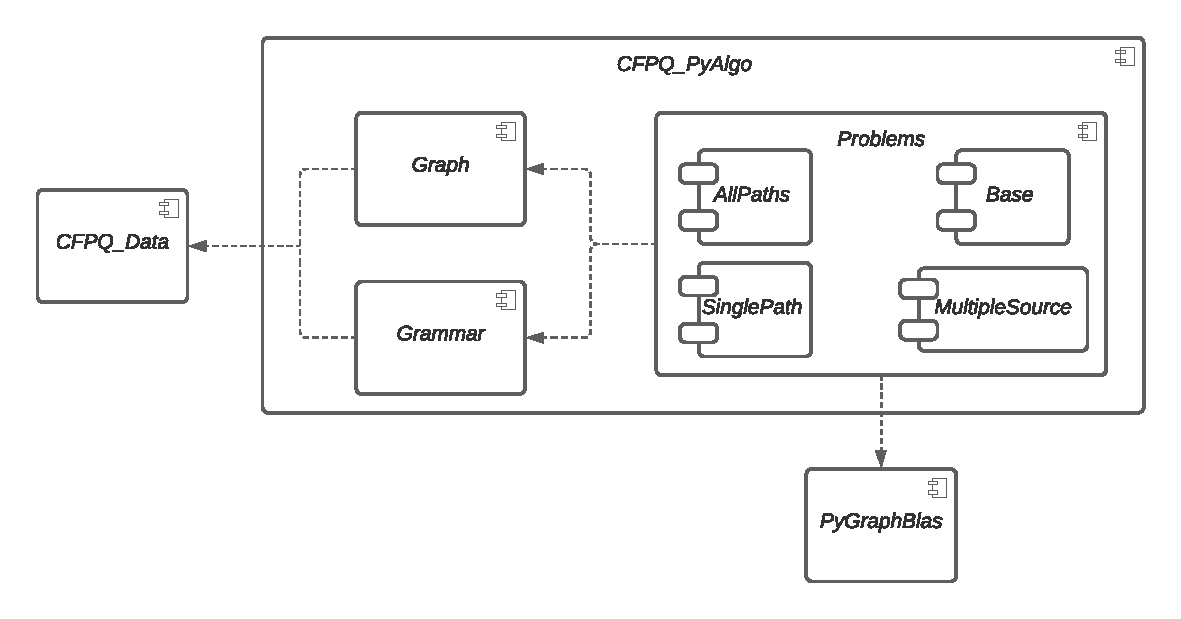
\includegraphics[scale=0.8]{img/pyalgo.pdf}
    \caption{Архитектура реализаций алгоритмов}
\end{figure}

Полученная архитектура \textit{CFPQ\_PyAlgo} состоит из трёх модулей: \textit{Graph}, \textit{Grammar} и \textit{Problems}. 

Модуль \textit{Graph} предназначен для представления графов и их загрузки в качестве входных данных. Модуль \textit{Grammar} реализует хранение и загрузку грамматики в виде ОНФХ, а также рекурсивного автомата. Оба модуля поддерживают данные из \textit{CFPQ\_Data}.

Модуль \textit{Problems} разбит на несколько частей. Создание каждой части мотивируется решаемой задачей. Все такие части содержат интерфейс задачи, который реализуют алгоритмы с использованием библиотеки \textit{PyGraphBlas}. В качестве входных данных реализации принимают путь до графа и путь до контекстно-свободной грамматики. Далее каждая конкретная реализация алгоритма выбирает нужные представления графа и грамматики из модулей \textit{Graph} и \textit{Grammar}, соответственно.

Разработанные алгоритмы из разделов 3 и 4 представлены в части \textit{AllPaths}, а из раздела 5 --- в \textit{MultipleSource}, исходный код которых находится в репозитории \textit{CFPQ\_PyAlgo}\footnote{Репозиторий \textit{CFPQ\_PyAlgo}: https://github.com/JetBrains-Research/CFPQ\_PyAlgo Дата посещения 13.05.2021}. Для предложенных реализаций написаны тесты на некоторые варианты входных данных и базовая документация. Репозиторий оснащен системой сборки и запуска тестов, а также в нем находятся скрипты для замеров производительности, результаты которых представлены в следующем разделе.

\section{Замеры производительности}
Рассмотрим результаты замеров производительности полученных реализаций. Для этого сначала опишем выбранные данные и окружение для постановки экспериментов.

\subsection{Окружение и данные для экспериментов}

Для постановки экспериментов над реализациями был использован ПК с операционной системой Ubuntu 20.04 и конфигурацией: Intel(R) Core(TM) i7-4790 CPU @ 3.60GHz CPU, DDR4 64 Gb RAM.

Из набора данных CFPQ\_Data были взяты графы следующих классов:
\begin{itemize}
    \item RDF --- реальные биологические данные;
    \item MemoryAliases --- графы анализа указателей языка Си. Обладают более сложной структурой в отличии от графов класса RDF.
\end{itemize}

Таким образом были выбраны графы, представленные в таблице 1.

\begin{table}[H]
\begin{center}
{

%\rowcolors{2}{black!2}{black!10}
\begin{tabular}{|l|c|c|}
\hline
Graph          & \#V       & \#E        \\
\hline
\hline
eclass\_514en  & 239 111    & 523 727   \\
enzyme         & 48 815     & 109 695   \\
geospecies     & 450 609    & 2 201 532 \\
go             & 272 770    & 534 311   \\
go-hierarchy   & 45 007     & 980 218   \\
taxonomy       & 5 728 398  & 14 922 125\\
\hline
arch           & 3 448 422  & 5 940 484 \\
crypto         & 3 464 970  & 5 976 774 \\
drivers        & 4 273 803  & 7 415 538 \\
fs             & 4 177 416  & 7 218 746 \\
\hline
\end{tabular}
}
\end{center}
\caption{Графы}
\end{table}
В качестве грамматик были взяты следующие:
\begin{itemize}
    \item $G_1: S \to \overline{sco} \ \ S \ \ sco\ \ | \ \ \overline{type} \ \ S \ \ type \ \ | \ \ \overline{sco} \ \ sco \ \ | \ \ \overline{type} \ \ type$
    \item $G_2: S \to \overline{sco} \ \ S \ \ sco \ \ | \ \ sco$
    \item $Geo: S \to bt \ \ S \ \ \overline{bt} \ \ | \ \ bt \ \ \overline{bt}$
    \item $MA:$
    \begin{itemize}
        \item $S \to \overline{d} \ \ V \ \ d$
        \item $V \to (S?\overline{a})^{*}S?(aS?)^{*}$
    \end{itemize}
\end{itemize}
Где $\overline{x}$ обозначает ребро обратное ребру с меткой $x$ в графе. Количество терминалов из выбранных грамматик, соответствующие меткам в графах, приведено в таблице 2.
\begin{table}[H]
\begin{center}
{

%\rowcolors{2}{black!2}{black!10}
\begin{tabular}{|l|c|c|c|c|c|}
\hline
Graph          & \#sco & \#type &\#bt & \#a  & \#d \\
\hline
\hline
eclass\_514en  & 90 512    & 72 517    &        ---        & ---  & --- \\
enzyme         & 8 163     & 14 989    &        ---        & ---  & --- \\
geospecies     & 0         & 89 062    &        20 867     & ---  & --- \\
go             & 90 512    & 58 483    &        ---        & ---  & --- \\
go-hierarchy   & 490 109   & 0         &        ---        & ---  & --- \\
taxonomy       & 2 112 637 & 2 508 635 &        ---        & ---  & --- \\
\hline
arch           &      ---     &  ---   &        ---        & 671 295 & 2 298 947 \\
crypto         &      ---     &  ---   &        ---        & 678 408 & 2 309 979 \\
drivers        &      ---     &  ---   &        ---        & 858 568 & 2 849 201 \\
fs             &      ---     &  ---   &        ---        & 824 430 & 2 784 943 \\
\hline
\end{tabular}
}
\end{center}
\caption{Количество терминалов из выбранных грамматик, соответствующих меткам в графах}
\end{table}

\subsection{Эксперименты над улучшением алгоритма построения индекса}

Сравнения реализации улучшения, предложенного в разделе 3, производились с реализацией базового алгоритма, основанного на произведении Кронекера, использующей тот же набор технологий и ПК для проведения экспериментов. 


В ходе проведения экспериментов было произведено 5 запусков с каждым графом и каждой грамматикой. В конце бралось среднее значение из каждой выборки. Таким образом результаты измерений представлены с $\pm \Delta = \pm 0,06$ сек точностью оценки при доверительной вероятности 0.95.

\begin{table}[H]
    \begin{center}
    %\rowcolors{4}{black!2}{black!10}
    \begin{tabular}{| l | c | c | c | c | c | c | c | c |}
      \hline

      \multirow{2}{*}{Name}  & \multicolumn{2}{c|}{$G_1$} & \multicolumn{2}{c|}{$G_2$} & \multicolumn{2}{c|}{\textit{Geo}} & \multicolumn{2}{c|}{\textit{MA}}\\
      \cline{2-9}
                      & Tns2   & Tns1   & Tns2 & Tns1 & Tns2  & Tns1  & Tns2    & Tns1 \\
      \hline
      \hline
      eclass\_514en   & 0.24   & 0.25   & 0.25 & 0.26 & ---   & ---   & ---     & ---\\
      enzyme          & 0.03   & 0.04   & 0.02 & 0.04 & ---   & ---   & ---     & ---\\
      geospecies      & 0.08   & 0.09   & $<0.01$ & 0.01 & 26.12 & 34.12 & ---  & ---\\
      go-hierarchy    & 0.16   & 0.19   & 0.23 & 0.29 & ---   & ---   & ---     & ---\\
      go              & 1.56   & 1.68   & 1.21 & 1.37 & ---   & ---   & ---     & ---\\
      pathways        & 0.01   & 0.02   & 0.01 & 0.01 & ---   & ---   & ---     & ---\\
      taxonomy        & 4.81   & 5.37   & 3.75 & 3.81 & ---   & ---   & ---     & ---\\
      \hline
      arch            & ---    & ---    & ---  & ---  & ---   & ---   & 262.45  & 390.05  \\
      crypto          & ---    & ---    & ---  & ---  & ---   & ---   & 267.52  & 395.98  \\
      drivers         & ---    & ---    & ---  & ---  & ---   & ---   & 1309.57 & 2114.16 \\
      fs              & ---    & ---    & ---  & ---  & ---   & ---   & 470.49  & 745.97  \\
      \hline
    \end{tabular}
    \end{center}
    \caption{Результаты экспериментов над улучшением построения индекса, время в секундах}
  \end{table}

В таблице 3 продемонстрировано время в секундах работы алгоритмов над графами в зависимости от грамматик. Знак "---" означает неприменимость грамматики к графу. Tns2 --- результаты алгоритма с улучшением, Tns1 --- результаты алгоритма без улучшения.

Таким образом, наблюдается всюду положительный результат. А именно, для графов типа RDF уменьшение времени выполнения составило до 23\%, а для графов MemoryAliases --- до 38\%. Особо выразительный выигрыш алгоритма с улучшением получился на графах типа MemoryAliases, так как в виду их сложной структуры происходит большое число действий при транзитивном замыкании в базовой версии алгоритма, а предложенное улучшение позволяет уменьшить число таких операций.

\subsection{Эксперименты над алгоритмом извлечения путей}

Для реализации предложенного алгоритма извлечения путей в разделе 4 было выбрано ограничение на глубину рекурсии в виде длины пути. Таким образом, к процедуре \textit{GetPaths} добавляется ещё один аргумент, который характеризует ограничение на длину пути, и в таком случае результатом будет набор путей длины меньше заданной этим аргументом.

В ходе эксперимента был выбран из таблицы 1 граф \textit{eclass\_514en} и грамматика $G_1$ и происходило восстановление путей из всех пар вершин, между которыми был обнаружен путь алгоритмом построения индекса, с ограничением на длину в 20 и 50. Сравнение происходит с алгоритмом, основанным на матричном умножении.

Таким образом были получены результаты, изображенные на рисунках 2 и 4, для предложенного алгоритма.
\begin{figure}[!]
\begin{minipage}[h]{0.49\linewidth}
\center{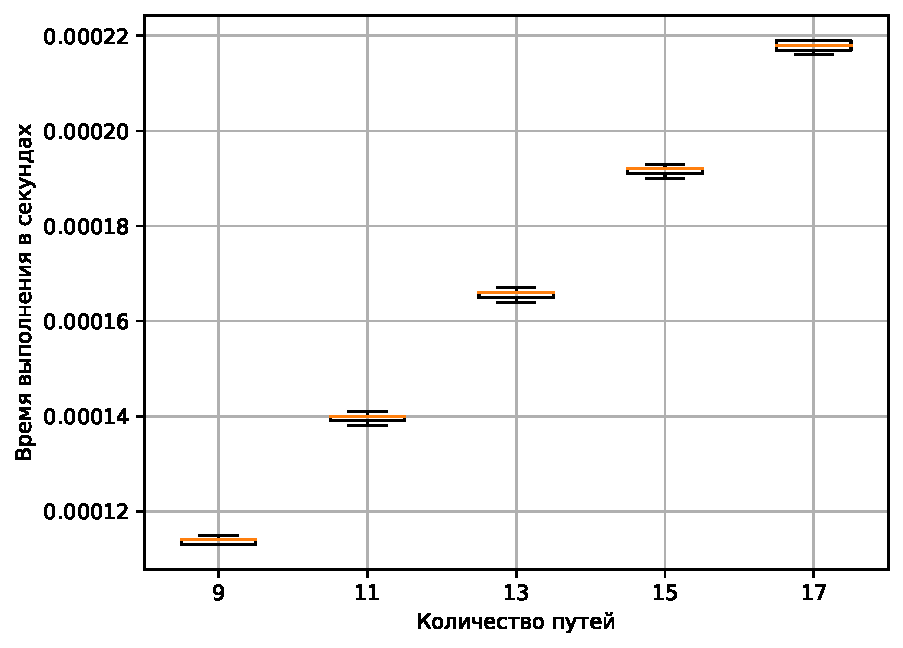
\includegraphics[width=8cm]{img/tensor_eclass_514en_20_small.pdf}}
\caption{Результаты эксперимента над извлечением путей Tns с ограничением по длине 20}
\end{minipage}
\hfill
\begin{minipage}[h]{0.49\linewidth}
\center{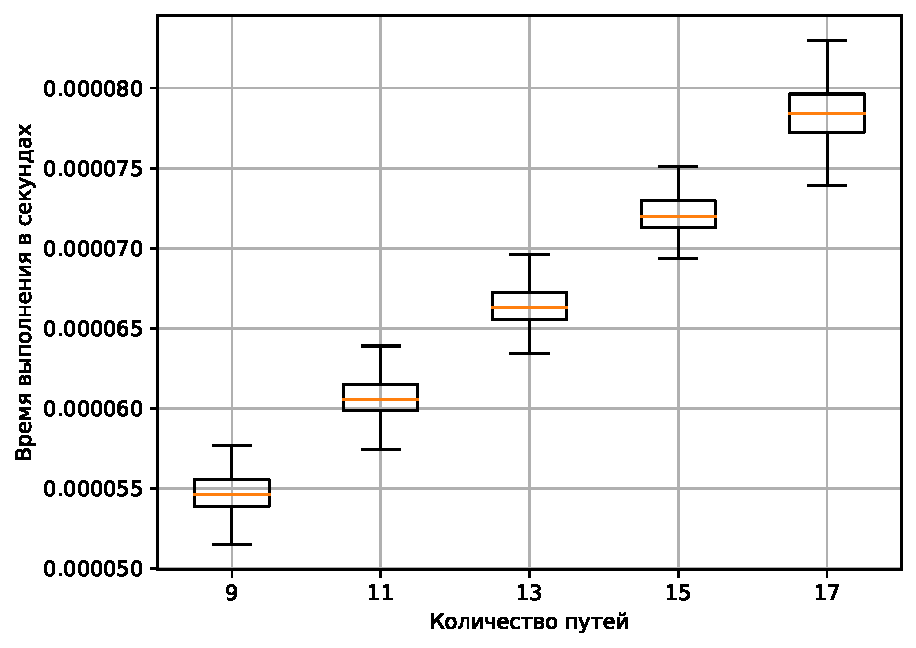
\includegraphics[width=8cm]{img/allMatr_eclass_514en_10_small.pdf}}
\caption{Результаты эксперимента над извлечением путей Mtx с ограничением по длине 20}
\end{minipage}
\end{figure}

На графиках приведены распределение времени для пяти самых часто встречающихся количеств найденных путей. Аналогичные результаты для алгоритма, основанного на матричном умножении, приведены на рисунках 3 и 5.

\begin{figure}[h!]
\begin{minipage}[h]{0.49\linewidth}
\center{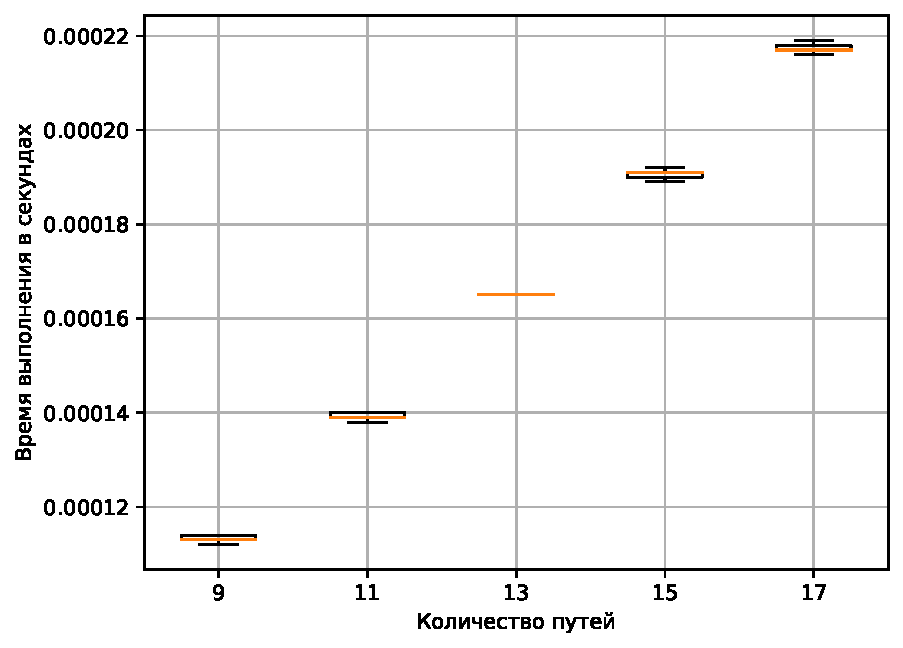
\includegraphics[width=8cm]{img/tensor_eclass_514en_50_small.pdf}}
\caption{Результаты эксперимента над извлечением путей Tns с ограничением по длине 50}
\end{minipage}
\hfill
\begin{minipage}[h]{0.49\linewidth}
\center{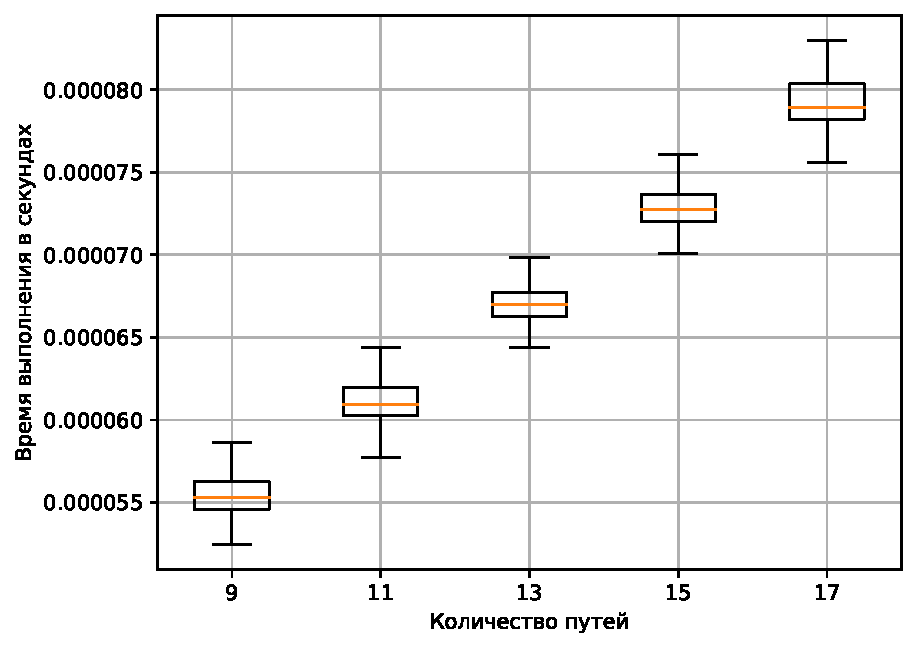
\includegraphics[width=8cm]{img/allMatr_eclass_514en_20_small.pdf}}
\caption{Результаты эксперимента над извлечением путей Mtx с ограничением по длине 50}
\end{minipage}
\end{figure}

На рисунках 2 и 4 наблюдается незначительный прирост времени выполнения при увеличении ограничения на длину путей.

Таким образом предложенный алгоритм медленнее аналога более чем в 100 раз по времени выполнения, так как в процессе обнаружения путей алгоритм, основанный на матричном умножении, строит структуру, которая явно хранит вершины, являющиеся частями искомых путей, в то время как для алгоритма, основанного на произведении Кронекера, приходится обходить матрицу смежности $C_3$.

\subsection{Эксперименты над алгоритмом обнаружения путей с заданным набором стартовых вершин}

Для постановки экспериментов над реализацией предложенного алгоритма в разделе 5 были выбраны из таблицы 1 графы \textit{go-hierarchy} и \textit{eclass\_514en} и грамматика $G_1$. Для каждого графа множество его вершин было разбито на непересекающиеся множества фиксированного размера. Далее производился запуск для каждого такого множества в качестве стартового набора вершин. Полученные результаты представлены на рисунках 6 и 7 синим цветом. Штрихом на диаграммах представлена медиана.

\begin{figure}[h]
\begin{minipage}[h]{0.49\linewidth}
\center{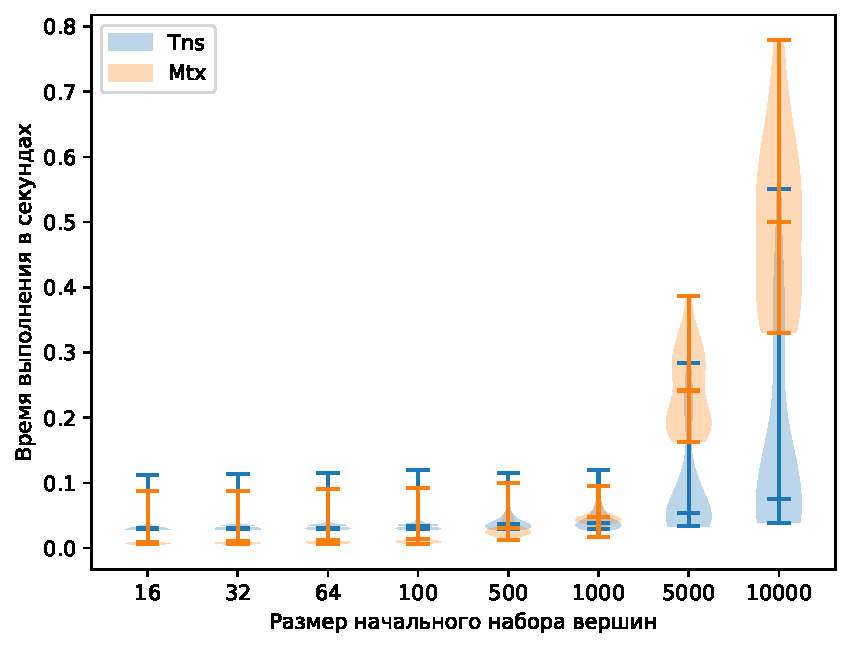
\includegraphics[width=8cm]{img/ms_all_eclass_514en_new.pdf}}
\caption{Результаты экспериментов над алгоритмом с начальном мн-вом вершин на графе \textit{eclass\_514en}}
\end{minipage}
\hfill
\begin{minipage}[h]{0.49\linewidth}
\center{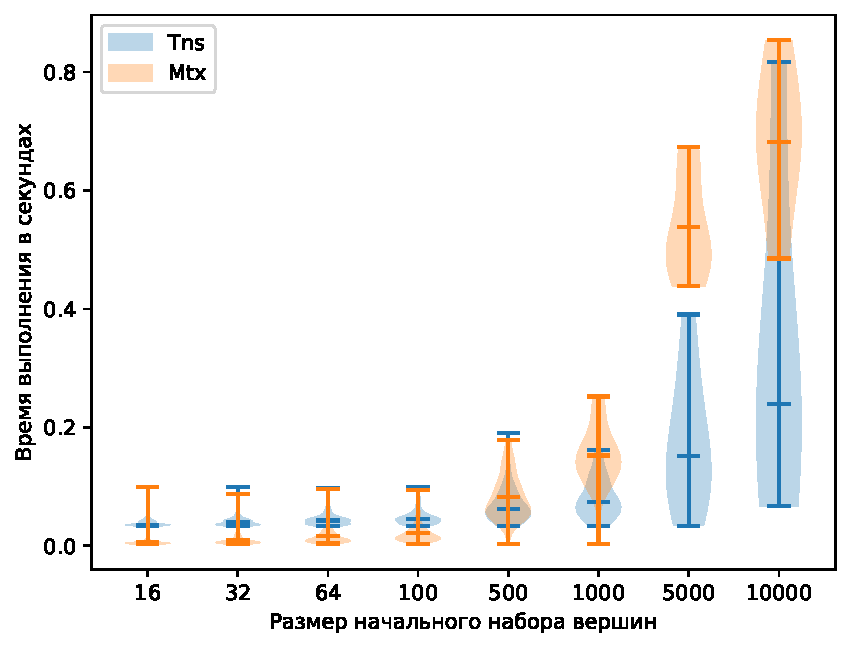
\includegraphics[width=8cm]{img/ms_all_go-hierarchy_new.pdf}}
\caption{Результаты экспериментов над алгоритмом с начальном мн-вом вершин на графе \textit{go-hierarchy}}
\end{minipage}
\end{figure}

Сравнение производилось с аналогичным алгоритмом через матричное умножение. Результат работы аналога представлен на рисунках оранжевым цветом.

Таким образом для взятых графов алгоритм через произведение Кронекера, сравним с аналогом на множествах начальных вершин размером не превосходящих 1000. Начиная с размера начального множества вершин 5000, алгоритм через произведение Кронекера демонстрирует меньшее время работы. Однако видно, что цель создания алгоритма с точки зрения времени выполнения оправдывается только при размере начального множества вершин меньше 1000. Так как в таблице 3 указано, что полную информацию о достижимости для графа \textit{eclass\_514en} можно получить за 0.24 с., а \textit{go-hierarchy} --- за 0.16 с.



% У заключения нет номера главы
\section*{Заключение}
В ходе работы были выполнены следующие задачи.
\begin{enumerate}
    \item Улучшен алгоритм построения индекса с использованием динамического пересчета некоторых шагов алгоритма и реализовано полученное улучшение.
    \item Разработан и реализован алгоритм извлечения путей по результату работы алгоритма построения индекса.
    \item Разработан и реализован алгоритм построения индекса с фиксированным набором стартовых вершин.
    \item Произведено экспериментальное исследование производительности реализаций. Полученное улучшение алгоритма поиска путей демонстрирует уменьшение времени до 38 \% по сравнению с версией без улучшения. Разработанный алгоритм с набором стартовых вершин быстрее существующего аналога. Однако алгоритм извлечения путей оказался медленнее до 100 раз того же аналога ввиду более сложно устроенных структур необходимых в процессе его работы.
\end{enumerate}

Также результат был изложен в статье "Context-Free Path Querying with All-Path Semantics by Matrix Multiplication", которая принята на конференцию GRADES-NDA 2021.

Реализации представлены в репозитории: \href{https://github.com/JetBrains-Research/CFPQ\_PyAlgo}{https://github.com/JetBrains-Research/CFPQ\_PyAlgo}.

% \nocite{*}
\setmonofont[Mapping=tex-text]{CMU Typewriter Text}
\bibliographystyle{ugost2008ls}
\bibliography{vkr}
\end{document}
